% ===== INICIO DEL PREÁMBULO =====
%
\documentclass[msc,oneside,a4paper]{udelar} % Poner msc para Maestría, dsc para Doctorado.
%
\usepackage[
acronyms, 											 %utiliza el glosario de acronimos.
nohypertypes={acronym,notacion,simbolos,glosario},   %quita los links en el texto al glosario.
%nonumberlist,                                       %quita los links en los glosarios al texto.
nogroupskip,                                         %quita los espacios entre diferentes grupos dentro de un glosario.	
nopostdot, 											 %quita el punto final en los acrónimos         .                           
]{glossaries}

\hypersetup{ colorlinks = true } % Hipervínculos: escribir "false" para imprimir o "true" para ver en digital.

% Ver los documentos de estilos bibliográficos para editar estas siguientes 2 líneas. Se deben de copiar a partir de los PDF de estilos bibliográficos y no es necesario que el estudiante las edite.
\usepackage{natbib} % Para algunos estilos bibliográficos
\bibliographystyle{estilos_bibliograficos/natbib/apalike}

\loadglossary % No comentar esta línea

% A su vez, la clase udelar.cls ya tiene los siguientes paquetes cargados automáticamente, que podrían ser de interés saber para el usuario:
% 
% {color},{hyphenat},{appendix},{lastpage},{babel},{inputenc},{amsmath,amssymb},{ifthen},{graphicx},{caption}
% {setspace},{tabularx},{eqparbox},{ltxcmds},{titletoc},{xcolor},{lineno},{xwatermark}

% Si se quieren agregar más paquetes, se recomienda colocarlos a partir de esta linea y antes de \begin{document}.
% ===========  INICIO PAQUETES ===============


% ===========   FIN PAQUETES   ===============

% Definición de correctores, con un máximo de tres correctores.
\definechangesauthor[color=redtex]{JLM}			% Siglas del primer corrector 
\definechangesauthor[color=bluetex]{JH}			% Siglas del segundo corrector
\definechangesauthor[color=greentex]{MC}		% Siglas del tercer corrector

% =====  FIN DEL PREÁMBULO  =====

% ===== INICIO DEL DOCUMENTO =====

\begin{document}
  %
  \title{Agentes cooperativos para vuelo inteligente de vehículos autónomos}
  %\subtitle{Subtítulo de la tesis}
  %\institutelogo{3} % Carga cantidad de logos seleccionados, con máximo de 3 logos.
  \author{Giovani}{Rondán}
  \author{Giovani}{Rondán}
  \author{Giovani}{Rondán}
  \escritura{en} % Se indica que el programa de Posgrado sea "en" o "de" tal área.
  %
  \director{Prof.}{Santiago}{Iturriaga}{D.Sc.}
  \director{Prof.}{Sergio}{Nesmachnow}{D.Sc.} % Comentar esta línea si se tiene solo un director de tesis.
  %\codirector{Prof.}{Nombre del 1er Codirector}{Apellido}{D.Sc.}  % Comentar estas líneas si no son necesarias.
  %\codirector{Prof.}{Nombre del 2do Codirector}{Apellido}{D.Sc.}
  %\codirector{Prof.}{Nombre del 3er Codirector}{Apellido}{D.Sc.}
  %\directoracademico{Prof.}{Nombre del Director Académico de Tesis}{Apellido}{D.Sc.}
  %
  \examiner{Prof.}{Nombre del 1er Examinador}{Apellido}{D.Sc.}
  \examiner{Prof.}{Nombre del 2do Examinador}{Apellido}{Ph.D.}
  \examiner{Prof.}{Nombre del 3er Examinador}{Apellido}{D.Sc.}
  \examiner{Prof.}{Nombre del 4to Examinador}{Apellido}{Ph.D.}
  \examiner{Prof.}{Nombre del 5to Examinador}{Apellido}{Ph.D.} % Comentar los que no son necesarios.
  %
  \graduatename{Ingeniería en Computación}
  \institute{Facultad de Ingeniería}{FIng}  % La primer institución es la principal.
  %\institute{Facultad de Medicina}{FMed}  % Agregar copias de esta línea para agregar instituciones.
  %\institute{Facultad de Agronomía}{FAgro}  % Agregar copias de esta línea para agregar instituciones. No se discrimina de que universidad es tal facultad.
  %\seconduniversity{Universidad XXXXX} % Se agrega el nombre de otra universidad. Comentar esta linea si no es necesaria.
  %\thirduniversity{Universidad YYYYY} % Se agrega el nombre de otra universidad. Comentar esta linea si no es necesaria.
  \graduatelocation{Montevideo}{Uruguay}
  %
  \date{10}{11}{2018} % Fecha del documento: día/mes/año
  % Palabras claves en español
  \keyword{1ra palabra clave}
  \keyword{2da palabra clave}
  \keyword{3ra palabra clave}
  \keyword{4ta palabra clave}
  \keyword{5ta palabra clave}
  % Palabras claves en inglés
  \foreignkeyword{1st keyword}
  \foreignkeyword{2nd keyword}
  \foreignkeyword{3rd keyword}
  \foreignkeyword{4th keyword}
  \foreignkeyword{5th keyword}
  %     
  \maketitle  % Comando que genera el título de la tesis.
  %
  \frontmatter  % Comando que genera la portadilla, el catalogo y el tribunal de evaluación. NO COMENTAR
  %
  \dedication{(Dedicatoria) A alguien cuyo valor es digno de ella.}


  \chapter*{Agradecimientos}

Quisiera agradecer a...

  \epigrafe{{\normalfont{(Epígrafe:)}} Frase que alude al tema de trabajo.}{Autor}


  \begin{abstract}

El presente trabajo constituye el estudio de algoritmos colaborativos de exploración y misiones de vigilancia sobre puntos predefinidos mediante una flota de drones capaces de operar de forma autónoma sobre escenarios con diversas características. La implementación de la solución al problema se basa en el paradigma de la computación basada en agentes. La misma está constituida por una máquina de estados encargada de resolver las distintas etapas por las que atraviesan los drones cuando ejecutan la misión, teniendo como objetivos el máximo cubrimiento de la zona a explorar en un tiempo óptimo de acuerdo a la duración de la batería de los drones, manteniendo vigilancia sobre puntos de interés previamente definidos e intentando mantener comunicación constante entre los drones de la flota. Una de las principales características de la solución implementada es que la misma es ejecutada por cada dron de forma autónoma, sin ninguna estación base que esté calculando rutas a seguir ni ningún otro tipo de decisión. El lenguaje de programación utilizado fue Python, las comunicaciones se manejan a través de conexiones TCP por medio de una red WiFi. Se utilizaron drones Parrot Bebop 2 para la investigación. Si bien la solución tiene en cuenta cuestiones específicas de las características de este modelo de dron, la misma es adaptable a cualquier otro.
Con el objetivo de validar el algoritmo implementado para la solución del problema se realizaron pruebas sobre distintos escenarios de exploración de áreas abiertas mediante simulaciones computacionales utilizando el simulador Sphinx. Se realizó la ejecución del algoritmo para diversas instancias de cada escenario con una flota de dos drones. También se realiza la ejecución de distintos tipos de algoritmos de modo de poder comparar los resultados experimentales. Como complemento se realiza la instalación y ejecución del algoritmo directamente en cada uno de los drones de modo de comprobar su correcto comportamiento en la realidad.
Los resultados obtenidos en la experimentación 
FALTA RESULTADOS GENERALES DE LOS RESULTADOS
La investigación concluye 
FALTA CONCLUSIONES GENERALES 
El trabajo realizado contribuye a presentar un desarrollo aplicable en la práctica que le permite a una flota de drones poder ejecutar tareas de exploración y vigilancia de puntos predefinidos de forma colaborativa y autónoma, maximizando el cubrimiento del territorio así como también optimizando la vigilancia sobre los puntos de interés elegidos.


\end{abstract}


  \begin{foreignabstract}

In this work, we present ...

\end{foreignabstract}
  %
%  \listoffigures	         % Lista de figuras
%  \listoftables	         % Lista de tablas
  \listadesimbolos 		     % Lista de símbolos
  %\listadenotaciones 	     % Lista de notaciones
  \listadesiglas 		     % Lista de siglas
  %
  \tableofcontents           % Tabla de contenidos. Compilar dos veces para ver los cambios completos.
  %
  \mainmatter % Comando que genera las listas y capítulos. NO COMENTAR
  %
  % Se incluyen los capítulos. Se pueden comentar los capítlos en los cuales no se está trabajando, para que el documento de trabajo sea más pequeño y compile más rápido.
  \chapter{Introducción}

El proyecto propone el estudio de distintos algoritmos colaborativos de inteligencia computacional basados en el paradigma de computación basada en agentes para determinar los patrones de exploración sobre un conjunto de vehículos (flota) capaces de operar de forma autónoma. La exploración es realizada sobre un escenario conocido a priori, teniendo los vehículos información sobre las áreas notables del mismo como son la presencia de puntos de interés y zonas inaccesibles para transitar. A su vez también se propone como objetivo simultáneo a la exploración la vigilancia de ciertos puntos del territorio previamente marcadas para dicho fin, llamados “Puntos de Interés” (POI por sus siglas en inglés), los cuáles pueden tener distinto tipo de prioridad de vigilancia asignados al iniciar la misión. Cabe destacar que la colaboración de los vehículos es llevado a cabo directamente entre los vehículos involucrados en la flota sin comunicarse con una estación base. Los vehículos utilizados en la investigación son vehículos aéreos no tripulados (UAV por sus siglas en inglés) conocidos comúnmente como drones. Al utilizar drones se tiene una limitante determinante para la exploración que es el tiempo de duración de una carga de batería. Al ser un trabajo colaborativo otra de las limitantes existentes es la calidad de la comunicación entre los drones, la cual puede verse afectada por diferentes aspectos como la distancia entre los mismos, condiciones atmosféricas, interferencias, etc. El objetivo de la exploración a realizar es el de cubrir la máxima proporción de territorio, realizarlo de forma tal de optimizar el tiempo de la misión debido principalmente a la limitante del tiempo de duración de la batería de los drones y con la capacidad de que los drones puedan continuar realizando la misión aunque hayan perdido la conectividad con el resto de la flota.
La motivación de este proyecto viene dada por el auge de la utilización de drones, principalmente los conocidos como vehículos aéreos no tripulados en diversos tipos de tareas y entornos. Dentro de las principales aplicaciones para el uso de drones no tripulados se encuentran las desarrolladas para tareas agrícolas [1], tanto en fertilización de campos como en mediciones, análisis del estado del suelo, de los cultivos, etc. También se encuentran aplicaciones muy controvertidas pero que cada vez son más utilizadas e importantes que son las aplicaciones militares [2]. Los drones no tripulados en aplicaciones militares son utilizados desde misiones de reconocimiento de zonas peligrosas, vigilancia [3] y apoyo en tareas de rescate  [4] hasta misiones de ataque de objetivos específicos (contando con drones que poseen armamento). 
Si bien existen distintos trabajos y estudios que refieren a la coordinación de drones para la realización de tareas, la mayoría de las aplicaciones que son llevadas a la práctica constan de drones pilotados de forma remota [4], donde es necesario contar con un piloto profesional certificado para conducir los vuelos, por lo que aún existe un amplio margen para estudiar soluciones a problemas donde los drones operen de forma autónoma y que puedan ser aplicables en la realidad. Para alcanzar los objetivos planteados en el estudio se analizan y comparan los comportamientos de los distintos algoritmos colaborativos mediante la ejecución de pruebas en simuladores. También se implementan y ejecutan los programas con los algoritmos desarrollados directamente en la flota de drones a modo de poder observar su comportamiento en la realidad.
En este documento se presentan los antecedentes encontrados y estudiados de forma previa a la realización del proyecto. A continuación se detallan las características de los drones utilizados, tanto a nivel de hardware como de software. Luego se describe la parte central del informe. En la misma se detallan las características de todas las herramientas utilizadas para el desarrollo del proyecto y se describe la máquina de estados implementada para la solución al problema. En la siguiente sección se describe la metodología para la experimentación, de describen los distintos casos de pruebas planteados y se analizan los resultados obtenidos. Finalmente el informe finaliza con el planteo de las conclusiones obtenidas en base a los resultados de la experimentación, incluyendo posibilidades de trabajo a futuro teniendo como punto de partida la investigación realizada.
 % Se carga el capítulo 01
  \chapter{Revisión de antecedentes}

Existen diversos antecedentes de investigaciones para la coordinación de un equipo de UAVs con el fin de completar tareas, motivados principalmente por fines militares.  En general estos antecedentes centran la formulación del problema en la monitorización de uno o varios objetivos determinados a priori como es el caso del siguiente estudio:

Frank Mufalli, Rajan Batta y Rakesh Nagi (2012)  [5]realizaron una investigación titulada “Simultaneous Sensor Selection and Routing of Unmanned Aerial Vehicles for Complex Mission Plans” que busca resolver el problema de optimizar tareas de investigación de instalaciones fijas, donde se conocen de antemano sus coordenadas, alternando entre los diferentes tipos de sensores con los que se equipan a las unidades UAV con las que se dispone para cumplir la misión, dado que cada instalación a investigar produce mejores o peores beneficios en función de que sensor lleva equipado el drone que la investigue.
El artículo utiliza como base para su desarrollo el TOP (team orienteering problem), el cual a su vez es una generalización de OP (orienteering  problem), que busca solucionar el problema de un vehículo que partiendo de un origen debe llegar a un destino previamente establecido.

Si bien los drones con los que se cuenta para el proyecto son similares, los mecanismos de selección para determinar cuál dron de la flota debe encargarse de un punto de interés en base a cuál obtiene el mayor beneficio puede adaptarse al problema planteado ya que los puntos de interés tendrán distintas prioridades lo que determina en cierto punto un beneficio mayor el de atender un punto con mayor prioridad.
Otro aspecto fundamental del proyecto es el tratamiento de las limitantes propias de los drones como lo son la duración de la batería y las comunicaciones entre los mismos. En base a esto encontramos los siguientes antecedentes de estudios: 

Cesare (2015)  [6] en su trabajo “Multi-UAV Exploration with Limited Communication and Battery” propone un algoritmo para la coordinación de un equipo de UAVs con el fin de explorar un territorio previamente desconocido, teniendo en cuenta las limitaciones que surgen por el tiempo de vuelo limitado de los drones por su batería y de los problemas que pueden surgir por problemas en la red que se utiliza para la comunicación del equipo. El mismo se basa en la premisa de que es aceptable que al finalizar la exploración no es necesario que todos los drones retornen al punto de partida.
El algoritmo definido por el autor se basa en una máquina de estados compuesta de cinco estados, siendo los mismos denominados explore, meet, sacrifice, relay y go home. Explore es el estado inicial de todos los UAV que forman parte del equipo y es aquí donde se define la estrategia de exploración del dron basándose la misma en definir fronteras entre el espacio explorado y el espacio desconocido. Después de un tiempo constante previamente definido se cambia al estado meet, donde el dron busca comunicarse con otro miembro del equipo para transmitir su información y a su vez actualizar la información interna que posee sobre las posiciones del resto de los drones; a su vez al comunicarse con otro miembro se negocia con el mismo quien pasa al estado relay y quien al estado sacrifice. Si se determina que el dron será sacrificado pasa al estado de exploración hasta que se calcule que le queda solo el tiempo suficiente de vuelo como para volver a encontrarse con el dron que se determinó que estará en estado relay, es entonces cuando cambia su estado a sacrifice y busca volver a encontrarse con el dron de estado relay para transmitirle la información que recolecto. En cambio el dron que fue seleccionado para después pasar a estado relay continúa su viaje volviendo al estado exploración, y cuando determina que le queda tiempo de vuelo suficiente solo para volver a la base aterriza para esperar al dron de estado sacrifice y finalmente retornar a la base cambiando al estado go home.

Este artículo provee un interesante enfoque sobre una arquitectura distribuida para la exploración de un territorio que en muchos puntos es similar al problema que se busca resolver en este proyecto, teniendo como principal diferencia la característica que se permite que no todos los miembros del equipo de UAVs retornen a la base.

Esten Ingar Grøtli y Tor Arne Johansen [7] en su trabajo “Path planning for UAVs under communication constraints using SPLAT! and MILP” desarrollaron un algoritmo basado en MILP para resolver el problema del offline path planning para múltiples UAVs. MILP es un algoritmo que optimiza una serie de variables basado en un sistema de ecuaciones y restricciones. En este paper el objetivo de los autores era desplegar los drones en una zona conocida para que sirvan de relés de comunicación entre estaciones aisladas. La parte central del algoritmo desarrollado se basa en resolver un MILP. Tomando en cuenta sus objetivos los autores definieron una función objetivo que determina rutas para los drones optimizando la conectividad entre los UAVs de la flota y minimizando el consumo de combustible. En resumen, los cuatro componentes principales de la función objetivo describen: el consumo de combustible para mantener la velocidad crucero, el consumo de combustible para acelerar y frenar, el consumo de combustible para cambiar de altitud y el nivel de conectividad entre los UAV de la flota. A su vez, las restricciones definidas en el MILP se usan para evitar colisiones, salirse de las zonas de vuelo autorizadas, entre otros controles. Este algoritmo de optimización es ejecutado en sucesivas iteraciones, en cada una alimentándose con datos de SPLAT!, un servicio para comunicaciones por radio que permite estimar el nivel de conectividad entre dos puntos en el espacio, lo cual permitió generar rutas progresivamente mejores con cada iteración. El proceso es repetido hasta que las rutas calculadas por el algoritmo cumplan con los requisitos de la misión que tengan que cumplir los drones, los cuales tienen que ser definidos de alguna forma matemática.
Los autores probaron su algoritmo con simulaciones y mostraron que produce rutas efectivas que se ajusta a una gran variedad de situaciones y obstáculos.

Si bien este artículo no está tan enfocado en la exploración sino en distribuir efectivamente los UAVs de una flota en un terreno, el enfoque de usar el MILP resulta muy interesante ya que puede ser adaptado a una multitud de situaciones incluyendo la de optimizar la exploración.

Ke Shang et al. (2014) [8] en su investigación titulada “A GA-ACO Hybrid Algorithm for the Multi-UAV Mission Planning Problem” desarrollaron un algoritmo híbrido que sirve para solucionar el problema de misiones de vigilancia con flotas de UAV, donde el problema se caracteriza dentro de uno de optimización combinacional. El algoritmo busca la planificación de rutas para los UAVs de modo que poder obtener el máximo beneficio en la vigilancia satisfaciendo la limitante de energía de los UAV. Se le considera algoritmo híbrido ya que utiliza la combinación de dos tipos diferentes de algoritmos: un algoritmo genético (GA, algoritmo evolutivo conocido) y un algoritmo de optimización de una colonia de hormigas (ACO). El problema está compuesto por objetivos de vigilancia los cuales deben ser visitados por la flota de UAV, donde cada uno de los objetivos provee de un beneficio de vigilancia determinado según su importancia. Las dos métricas utilizadas para medir la eficiencia y eficacia del algoritmo son la suma total de beneficios de vigilancia obtenidos y el tiempo de la misión. El problema planteado es modelado por los autores mediante un grafo conectado donde los nodos son los objetivos a visitar (0=nodo inicial, n=nodo final), cada arista entre nodos representa un camino entre ellos y donde cada objetivo tiene asociado un beneficio de vigilancia particular. El objetivo del algoritmo es encontrar m caminos empezando y terminando desde los nodos inicial y final visitando los objetivos de modo de maximizar el beneficio de vigilancia. Cada nodo se puede visitar como máximo una sola vez. La restricción aplicada es un tiempo máximo de duración de la misión que depende de la energía restante de los UAV de la flota. 
En cuanto a la especificación del algoritmo híbrido implementado por los autores, se distinguen responsabilidades distintas para cada algoritmo de forma individual: mientras que el algoritmo genético es el encargado de intentar mantener y evolucionar una población (en este caso de nodos objetivos a visitar) hacia una mejor solución, el ACO iterativamente permite que las hormigas (en este caso los elementos de la flota de UAV) dejen un rastro con feromonas para encontrar mejores soluciones. El algoritmo propuesto incorpora ambas habilidades de mejoras de los dos algoritmos anteriores donde la innovación está dada por la suplantación de malos individuos de la población por nuevos generados por el ACO la cual mejora la calidad de la solución a medida que se incrementan las iteraciones. Los resultados obtenidos mediante simulación muestran que el algoritmo planteado ofrece beneficios similares o mejores que los máximos ofrecidos por los restantes algoritmos comparados mientras que en cuanto al tiempo ofrece un tiempo promedio aceptable para su aplicabilidad.

Con el estudio anterior se pueden obtener ciertos aspectos definidos los cuales pueden utilizarse en el proyecto como por ejemplo la forma de caracterizar la eficiencia y eficacia del territorio a recorrer más allá del cubrimiento. Un aspecto diferencial entre ambos estudios es que el realizado por Ke Shang et al. (2014) no considera el problema de la limitante en la conexión entre los drones.

En relación al problema específico del manejo de la comunicación entre los drones de la flota resaltamos los siguientes estudios:

Schleich et al. (2013) [9] en su trabajo “UAV Fleet Area Coverage with Network Connectivity Constraint” desarrollaron un modelo de cubrimiento de áreas para una flota de drones no pilotados con la restricción de mantener la mayor conectividad posible entre los mismos y con una estación base. El modelo introducido se basa en la selección de las rutas a tomar por los drones mediante el comportamiento por feromonas. Los autores introducen cuatro métricas para la evaluación de su modelo y comparan los resultados obtenidos contra un modelo de selección aleatoria de las rutas. El trabajo resalta la capacidad que tiene una flota de drones en misiones de reconocimiento, exploración y vigilancia ya que ofrece teóricamente la posibilidad de duración ilimitada de la misma ya que un subconjunto de la flota puede estar recargando sus energía mientras el resto continúa con la misión. El escenario propuesto implica el mantenimiento de una red ad-hoc entre los drones de la flota así como también la obtención de medidas de forma simultánea del área a explorar en al misión. Las cuatro métricas introducidas por los autores con las que se comparan los distintos modelos son: velocidad de cubrimiento del área, exhaustividad del cubrimiento del área, confiabilidad del cubrimiento y el mantenimiento de la conectividad. Para obtener valores para las métricas se divide el área a explorar en pequeños rectángulos de largo y ancho determinado de modo que cada vez que un dron pasa por esa área se manda un aviso a los drones conectados y a la base. El modelo de cubrimiento de área desarrollado cuenta de tres etapas secuenciales: selección del dron vecino al cual se intenta estar conectado, cálculo de la ruta alternativa viable para dónde debe dirigirse y la aplicación del comportamiento basado en feromonas para seleccionar la mejor ruta basado en los cálculos anteriores. Los resultados obtenidos por los autores en cuanto a las métricas medidas fueron buenos para el modelo presentado cuando la flota de UAV´s tenía un número generalmente mayor a 20 nodos. En cuanto a conectividad entre la flota y porcentaje de nodos conectados a la base obtuvo mejores resultados que los otros modelos, manteniéndose relativamente similar en cuanto al resto de las métricas.
Si bien el estudio ataca una de las limitantes principales del proyecto como lo es la conectividad entre los drones, en este caso se evalúa la calidad de la conexión en relación a cuántos drones están conectados a una estación base, característica que no se tiene en la investigación actual. En el caso de las métricas planteadas por los autores para evaluar la calidad de la misión, las mismas son aplicables al proyecto actual adaptando la medida de conectividad al contexto planteado.

I. Bekmezci et al. (2013) [10] , en su investigación “Flying Ad-Hoc Networks (FANETs): A survey, Ad Hoc Network.”, presentan en su artículo una nueva denominación para la familia de redes ad hoc encargada de la comunicación en sistemas multi UAV el cual denominan “Flying ad hoc Network (FANET)”. También presentan una definición para este tipo de familia, una comparación con familias existentes como lo son las MANETs (Mobile ad hoc Network) y VANETs (Vehicle ad hoc Networks), desafíos en el diseño de las FANET, escenarios donde aplique el uso de FANET, distintos protocolos utilizados en ellas, investigaciones abiertas, etc, mediante la recopilación de distintos artículos de la literatura. A través de esta recopilación de la literatura existente sobre las FANET, los autores presentan estudios que focalizan en distintas áreas de las FANET como las características de diseño de las mismas, consideraciones al diseñarlas y distintos tipos de protocolos existentes en las FANET. Finalmente se mencionan estudios donde se generen resultados a través de simulaciones de las distintas áreas mencionadas.
Inicialmente se presentan los problemas que surgen al utilizar un pequeño grupo de UAVs para una misión particular. Entre los más importantes está el problema del diseño la infraestructura necesaria para la comunicación entre los distintos UAVs. Los autores mencionan dos enfoques utilizados en la literatura: comunicación a través de una infraestructura entre los UAV con una estación base y otro enfoque de comunicación entre los distintos UAV directamente mediante una red ad hoc generada entre ellos. Las características principales de los elementos de una FANET según la literatura presentada son las siguientes: gran movilidad de los nodos y gran distancia entre ellos, topología de la red muy cambiante y nodos que deben soportar tanto una comunicación peer-to-peer como también recolectar información del entorno mediante sensores. En el artículo se mencionan distintos escenarios en donde se puede aplicar el concepto de una FANET. Entre ellos se destacan escenarios donde se desee extender la escalabilidad de una misión con multi UAVs en los que generalmente no existe o no se puede comunicar con una estación base (debido a las grandes distancias entre los nodos y la base por ejemplo), escenarios donde se necesite una comunicación multi UAV confiable, escenarios de enjambres de UAVs (para evitar colisiones entre ellos por ejemplo), etc.
Dentro de las características en el diseño de una FANET, se mencionan los siguientes puntos: nodos con gran movilidad y con gran velocidad lo que lleva a que las FANET tengan que recalcular continuamente las rutas de vuelo de los UAV, baja densidad de los nodos con mucha distancia entre ellos, cambios rápidos y continuos en la topología de la red (debido a la movilidad y/o fallas en los nodos), poder computacional en general limitado por el tamaño de los UAV, localización en general a través de GPS en cada UAV, etc.   
Luego los autores hacen referencia a estudios donde se focalizan las consideraciones a tener en cuenta para el diseño de una FANET, de las que se destacan: adaptabilidad a entornos diversos y cambiantes, escalabilidad para poder aplicar los algoritmos con cualquier cantidad de UAVs, latencia mínima en el envío de paquetes entre los UAV, limitantes impuestas por el hardware de las UAV y un ancho de banda necesario para el envío de la información obtenida por los UAV.
Como último ítem importante los autores destacan los distintos protocolos de comunicación en una FANET recopilados en la literatura. Se observa que se dividen de acuerdo a la capa de red donde aplican los protocolos. Encontramos en la capa física dos tipos de modelos: el modelo de propagación de ondas de radio y el modelo de estructura de antena. Tenemos en la capa MAC principalmente el protocolo IEEE 802.11 como el más utilizado. En la capa de red se observa de los estudios que se utilizan generalmente protocolos de ruteo provenientes de las MANET. Sin embargo una estrategia de ruteo basada solamente en información de la locación de los nodos puede satisfacer las necesidades de una FANET. En la capa de transporte los estudios mencionan que la responsabilidad más grande de los protocolos es la de la confiabilidad en el transporte de los paquetes, control de flujo y control de congestión de los mismos.
Los estudios mencionados en la sección de simulaciones presentan como las distintas implementaciones de soluciones para resolver los problemas típicos de las FANET llevan a resultados aceptables, dejando también muchos campos de investigación abiertos.

El artículo otorga una visión global del problema de diseño de una red ad hoc entre UAVs, el estado actual de investigación en el área y permite relevar algunos estudios realizados en áreas específicas del problema planteado, permitiendo un mayor entendimiento de a que se enfrenta cuando se quiere diseñar una red ad hoc entre UAV. Se considera este artículo de gran valor por la gran recopilación de la literatura disponible.
Como último antecedente que trata sobre el problema de la comunicación entre drones dejamos planteados los principales conceptos desarrollados en el capítulo 66 del libro “Handbook of Unmanned Aerial Vehicles” escrito por los autores Andrew Kopeikin, Sameera S. Ponda y Jonathan P. How [11] .


El capítulo busca analizar las tecnologías existentes sobre control de comunicación por red en equipos de UAVs. Dado que los UAVs son móviles, las comunicaciones en estas redes son casi exclusivamente inalámbricas y en general buscan transmitir la información hacia una central donde la información se procesa. También se busca en general que los diferentes UAVs puedan comunicarse entre ellos de forma que puedan actuar en conjunto. La calidad de una red se puede evaluar en función a su topología, es decir su configuración de enlaces entre nodos y la calidad de estos. Existen varios mecanismos de control que permiten mejorar la calidad de una red de UAVs, la mayoría se traducen básicamente a implementar una o varias de estas acciones:
Posicionar los UAVs de forma que se reduzca la distancia entre ellos
Aumentar la potencia de los transmisores, o eligiendo ubicaciones especialmente favorables para la transmisión
Eligiendo activamente las conexiones habilitadas en una red y determinando caminos óptimos dentro de la red
Aumentando la cantidad de UAVs en la red

Los principales desafíos que una red inalámbrica tiene que superar son la distancia entre los nodos y la interferencia provocada ya sea por obstáculos físicos o por el ruido de otras señales. Los UAVs aéreos en general funcionan en cielo abierto y eso les permite evitar la mayoría de estos problemas, aunque no siempre. Hay situaciones donde los UAVs deben volar en zonas urbanas o a baja altitud y eso acarrea problemas. De esta forma el objetivo que se le quiere dar a la red y el tipo de vehículo que se va usar en ella es fundamental para decidir su diseño. La potencia de los transmisores del UAV puede verse limitada por el consumo de energía que representan, por el espacio que ocupan, o porque otros instrumentos del UAV pueden ser de mayor prioridad (incluyendo la CPU).
La arquitectura de la red depende en gran parte del tipo de información que se quiere enviar a través de ella. Una red de UAVs debe tener esto en cuenta ya que puede usarse para transmitir una gran variedad de datos, aunque básicamente se los puede subdividir en dos clases:
Mensajes de control y comandos. Estos pueden dar órdenes a los UAVs, transmitir telemetría básica sobre el estado del UAV (como su posición, cantidad de batería, etc). Estos mensajes requieren poco ancho de banda pero no son resistentes a fallos y pueden requerir un bajo delay.
Información captada por los sensores del UAV. Estos pueden ser imágenes, video, audio, datos complejos, etc. Requieren un mayor ancho de banda y tienen los mismos requerimientos que si fueran a ser transmitidos por Internet.

La topología de una red puede definirse fácilmente como un grafo G=(V,E) pero también como una matriz de adyacencia A tal que aij = 1 si hay una conexión entre los nodos i y j, y 0 en otro caso. Una de las representaciones más comunes es la de la matriz Laplaciana: 
Donde A es la matriz de adyacencia y D es la matriz diagonal tal que:
Los valores propios de esta matriz cumplen con la propiedad:
Y en particular  es conocido como la conectividad algebraica del grafo y determina la velocidad de convergencia en la mayoría de los algoritmos de toma de decisiones por consenso, por lo que muchos algoritmos intentan maximizar este valor. De todas formas hay que indicar que orientar el algoritmo de consenso únicamente a maximizar  no resulta una buena idea ya que se corre el riesgo de que los UAVs se centren demasiado en mejorar la conectividad entre ellos y no en cumplir con su verdadero objetivo.
 % Se carga el capítulo 02
  \chapter{Características de hardware}


\section {Drones}
La investigación toma como base los drones Parrot Bebop 2 [12], los cuales son usados principalmente por público general con fines recreativos. Debido a esto poseen un diseño resistente y simple, además de contar con una cámara de buena calidad, GPS y sistemas de estabilización de vuelo. Estas características resultaron de utilidad a la hora de desarrollar la aplicación.
Sin embargo, este modelo también plantea serias limitaciones, en particular, no es un modelo que esté pensado para que ejecute programas por su propia cuenta. Si bien existe un SDK provisto por Parrot que permite programar al dron, todas las aplicaciones existentes se basan en controlarlo a distancia, ya sea por medio de una computadora o un smartphone. La aplicación más notable que existe para los Bebop 2 es FreeFlightPro [13], una aplicación para smartphones que le permite a los usuarios controlar el dron de forma manual. La falta de aplicaciones que ejecutan su código desde el dron mismo se debe en gran parte a su sistema operativo y a su arquitectura ARM7. Los Bebop 2 vienen de fábrica con un sistema operativo embebido Unix BusyBox [14], el cuál está configurado para limitar lo más posible a los usuarios que intenten realizarle modificaciones al dron. Entre otras limitaciones los Bebop 2 no pueden conectarse a Internet, solo permiten el acceso a una parte limitada de la memoria y no pueden instalar o compilar programas nuevos. Esto último resulta especialmente problemático ya que obliga a compilar los programas en otros sistemas y la arquitectura ARM7 implica que solo se pueden usar algunos dispositivos específicos para compilar los programas que se quieren instalar en el dron. En futuras secciones se discutirán las soluciones propuestas por el equipo para superar estas limitaciones y la influencia que tuvieron sobre el proyecto en general.
A continuación se describen las principales especificaciones del dron [15]:

\begin{table}[h!]
	\centering
	\caption{Características del dron Parrot Bebop 2.}
	\label{tab:comp}
	\begin{tabular}{|c|c|}
		\hline
		Característica & Descripción\\
		\hline
		Sistema de rotores & Cuatro rotores, tres hojas por cada hélice - 5 centímetros de diámetro -. Son de plástico flexible, bastante resistentes y fácilmente reemplazables \\
		Velocidad máxima horizontal & 18m/s \\
		Velocidad de ascenso máxima & 6m/s \\
		Alcance de señal & 300 metros \\
		Batería & 2.700 mAh \\
		Autonomía & 25 minutos de vuelo \\
		Cámara & 14 megapíxeles \\
		Dimensiones & 33 x 30 x 10 centímetros \\
		Memoria (accesible por usuarios) & 8GB \\
		Peso & 480 gramos \\
		Sistema Operativo & Linux (Busybox) \\
		Arquitectura de CPU & ARMv7 \\
		Sensores (accesibles vía el SDK) & Cámara digital (1080pi)
		Sensor GPS
		Sensor de altura (ultrasonido) \\
		Sensores (no accesibles vía SDK) & Acelerómetro
		Giroscopio \\
		\hline
	\end{tabular}
\end{table}




\section {Simuladores}
Para evaluar y testear los programas desarrollados en este proyecto era necesario usar simuladores ya que no resulta conveniente probar código en desarrollo en un dron real. Esto permite proteger tanto al dron como a las personas que se encuentren en la cercanía. También ayuda a la hora de realizar la evaluación experimental ya que permite realizar pruebas automatizadas de forma eficiente. 

Se optó por usar Sphinx [16], el simulador para drones oficial de Parrot. Sphinx es un simulador basado en el software de robótica Gazebo para ambientes linux de 64 bits, y una tarjeta gráfica con soporte de OpenGL 3.0. En caso de querer hacer uso de la cámara frontal del dron es recomendable contar con una tarjeta gráfica GeForce 1060 Ti o superior. Parrot también provee firmwares que simulan modelos específicos de sus drones, incluyendo el Bebop 2, que se pueden cargar en Sphinx.
Sphinx también permite crear mundos (entornos de simulación) y drones por medio de archivos de configuración. Para agregar varios drones a la simulación se editan estos archivos, donde además es posible determinar las características de los mismos, incluyendo su cámara y su batería.
Es posible configurar los drones simulados para que se apropien de una interfaz wifi con la que cuente el equipo sobre el que se ejecuta la simulación para así poder enviarle órdenes. Además cada dron en la simulación genera una interfaz virtual por la que también se puede establecer la comunicación.
Sphinx facilita el desarrollo de aplicaciones para drones, pudiendo optar entre distintas opciones de desarrollo como lo son el SDK [17] de Parrot u otras librerías de terceros como pyparrot [18].    
La principal desventaja del simulador es que requiere muchos recursos de GPU para ejecutar las simulaciones: en general las computadoras de las que disponía el equipo no podían soportar más de 2 drones simulados a la vez. Además, Sphinx presenta serios problemas a la hora de simular varios drones en la misma instancia del programa, en particular los comandos que controlan el movimiento de los drones no funcionan de forma apropiada. Esto se pudo solucionar ejecutando cada dron en una instancia separada de Sphinx, sin embargo esta solución agrava el problema del consumo de recursos.
Para poder simular una mayor cantidad de drones es posible utilizar varias computadoras conectadas en una misma red, cada una con sus propios drones simulados estableciendo un canal de comunicación entre las computadoras. % Se carga el capítulo 03
  \chapter{Implementación}
El desarrollo del proyecto se llevó a cabo a través de una serie de etapas las cuáles se detallan a continuación. Las mismas incluyen distintos aspectos tales como descripción de las herramientas utilizadas (hardware y software), configuración necesaria de las mismas, implementación de la solución y finalmente experimentación con casos de prueba, incluyendo análisis de los resultados obtenidos.

\section {Autonomía de los drones}
Uno de los objetivos del proyecto es poder ejecutar la solución implementada de forma nativa en cada uno de los drones de forma tal que la flota pueda volar autónomamente sin la necesidad de una estación base que se esté en comunicación con ellos. En las siguientes secciones se detalla el trabajo realizado para cumplir con esta meta. 
\section {Herramientas de compilación}
El primer desafío encontrado fue el de implementar una solución que pueda ejecutarse en la arquitectura ARMv7 [19] que posee el dron Parrot Bebop 2, teniendo en cuenta que los equipos donde se desarrolla la solución están basados en la arquitectura x86 de los procesadores Intel.

Se plantean diferentes alternativas para solucionar este problema. La primera es la de realizar un cross-compile. Se entiende por cross compile la acción de compilar código en un sistema huésped que no tenga la misma arquitectura que el sistema objetivo en el cual se piensa ejecutar el programa, de esta forma se genera un ejecutable compatible con la arquitectura del sistema destino. En este proyecto, el sistema huésped son computadoras comunes de arquitectura x86 y el sistema destino es el dron con arquitectura ARMv7. Esta opción también incluye la utilización de compiladores específicos para la arquitectura de destino seleccionada. 

La segunda alternativa es la de utilizar el emulador Qemu [20-21] que permite la ejecución de sistemas operativos diseñados para arquitecturas diferentes a los del sistema anfitrión.
Por medio de Qemu es posible emular la arquitectura del dron, por lo que al momento de compilar no es necesario hacer uso de la técnica de cross compile dado que el ejecutable generado con la compilación por defecto va a ser compatible con el dron.

Como tercera opción se plantea utilizar una CPU que posea arquitectura ARM para que de ese modo, utilizando el mismo planteo que con el emulador Qemu, se pueda compilar directamente en la arquitectura destino sin necesidad de realizar el cross compile. Una de las opciones de CPU con arquitectura ARM más accesibles en el mercado es el de los dispositivos Raspberry Pi [22], los cuales permiten realizar todas las mismas acciones que con un PC tradicional.

Al momento de analizar las distintas alternativas se decidió utilizar la Raspberry Pi para compilar directamente en ella en lugar de hacer cross compile [23] o utilizar el emulador Qemu. Cross compile genera dificultades al momento de compilar cuando las librerías a utilizar (como por ejemplo el sdk del dron) requieren de muchas dependencias. Qemu, si bien otorga las mismas funcionalidades que la Raspberry Pi, tiene una complejidad mayor en cuanto a instalación y posterior configuración.
De todas formas, compilar e instalar en el dron resulta bastante complejo y consume mucho tiempo, por lo que se intentó minimizar la cantidad de programas a instalar en el dron.
\section {Lenguaje de programación}
Una de las tareas básicas para poder implementar una solución de este tipo es la de poder comunicarse con los drones mediante código en algún lenguaje de programación con el objetivo de darles órdenes para que realicen las acciones necesarias (despegue, aterrizaje, movimientos, etc). Existe un sdk oficial provisto por Parrot que permite realizar este tipo de tareas y que está disponible para distintos lenguajes de programación como C, Java, Objective C. Mediante el sdk se pueden realizar programas en cualquiera de estos lenguajes para darles órdenes a los drones pero con la limitante de que están pensados para que sean ejecutados en una terminal distinta al dron, ya sea una pc, smartphone, tablet, etc. Además, todos estos lenguajes son compilados.

Tanto en C, como en Java y Objective C se debe realizar una tarea de cross compile para ejecutar los programas en el dron o utilizar un intermediario como la Raspberry Pi y se debe hacer cada vez que se modifica el programa. Esto va en contra del principio establecido anteriormente de minimizar los cross-compiles. La solución a este problema vino dada por utilizar una librería para el lenguaje de programación Python llamada pyparrot la cual implementa una interfaz para el sdk oficial de Parrot. Python es un lenguaje de programación de scripting por lo que no es necesario compilar los programas desarrollados. Lo que se debe compilar es el intérprete de Python y algunas librerías que están escritas en C, sin embargo esto hay que hacerlo una única vez y luego se puede desarrollar el resto del programa sin tener que hacer más cross-compiles. De esta forma se procedió a usar la Raspberry Pi para generar ejecutables del intérprete de Python en ARM7. Finalmente se instaló esta versión compilada de Python en cada uno de los drones de forma que cada uno pudiese ejecutar de forma nativa los scripts en dicho lenguaje de programación. Esto permitió que se pudiese desarrollar el código directamente en equipos que no tuviesen arquitectura ARM y ejecutarse en el dron sin necesidad de realizar ninguna configuración extra.

\section {Conectividad entre los drones}
Como ya se mencionó, uno de los principales objetivos del proyecto es el de crear una flota de drones que sea completamente autónoma, es decir, que no necesite ningún equipamiento extra para funcionar. Por esta razón la primera opción para crear una red de comunicación entre los drones era la de crear una red ad-hoc. En una red ad-hoc todos los nodos de la red se encuentran en igualdad de condiciones (es decir que no hay un nodo central) y los nodos pueden seguir operando sin tener necesidad de estar conectados a toda la red (según el programa puede que ni siquiera sea necesario mantener una conexión con la red todo el tiempo). En el caso particular de la exploración de una zona con una flota de drones esto plantea varias ventajas. En primer lugar las redes ad-hoc permiten que los drones individuales sean completamente autónomos entre sí, incluso pueden seguir trabajando habiendo perdido toda conexión con el resto de la red (si bien esto implica que probablemente van a realizar su trabajo de forma menos eficiente). Además los drones pueden servir de relés para otros drones, por ejemplo, puede suceder que dos drones se encuentren muy lejos entre sí como para establecer una comunicación directa pero si existe un tercer dron que se encuentre en un punto intermedio entre ellos este puede servir de relé entre los dos. Esto aumenta de forma considerable el alcance que puede tener la red, lo cual aumenta el tamaño del área que se puede explorar de forma efectiva.

Debido a las ventajas descritas se analiza la posibilidad de implementar una red ad-hoc en los drones Bebop 2 pero los mismos no cuentan con una  tarjeta de red con soporte para el modo ad-hoc con la configuración por defecto. 
El modelo de la  tarjeta de red integrada en el dron es Broadcom BCM4360 [24], la cual en la configuración por defecto en los drones no permite asignar otros modos de conexión a la interfaz wifi distintos a Master y Managed. Los Bebop 2 vienen de fábrica con su interfaz configurada en modo Master, de esta forma cada dron publica su propia red wifi a la cual se pueden conectar otros dispositivos como teléfonos celulares o computadoras. Esta es la forma en la que los usuarios controlan a los drones normalmente.
Se investigó la posibilidad de incorporar modificaciones a los drivers que trae por defecto el dron pero la instalación de los mismos no es posible realizarla sin incorporar modificaciones riesgosas sobre el sistema operativo BusyBox que en caso de fallos puede llevar a errores irreparables en el funcionamiento del mismo. Debido a estos inconvenientes se determinó descartar la configuración de la red ad-hoc.

Finalmente se decidió usar en su lugar una red wifi. Este enfoque tiene algunas desventajas con respecto a las redes ad-hoc, la más importante es que en una red wifi los drones dependen de una infraestructura externa a ellos que mantenga la red. Sin embargo esta infraestructura no tiene porqué ser muy compleja, puede componerse por módems portátiles y routers ubicados en lugares estratégicos para cubrir la zona. Incluso puede llegar a componerse por teléfonos celulares.
Por otra parte, una red wifi tiene un alcance mucho mejor definido, por lo que resulta más fácil evitar las pérdidas de conexión con la red.
Además, un dron conectado a la red debería ser capaz de establecer conexiones con cualquier otro dron conectado, sin importar la distancia entre ellos. Esto permite establecer comunicaciones a gran distancia sin necesidad de recurrir al uso de otros drones como relés, que si bien es una técnica muy útil, también resulta más difícil de gestionar.

Para implementar esta red en los drones hubo que realizar ciertas modificaciones en su configuración. En primer lugar se cambió el modo de la interfaz a Managed, para que todos los drones puedan estar conectados a la misma red. Luego se le configura a cada uno una dirección IP, el nombre del Punto de Acceso y su contraseña. Para que esta configuración no interfiera el funcionamiento por defecto del dron con aplicaciones que desean conectarse a su interfaz wifi se instala un script en el mismo que permite cambiar el modo de la interfaz al presionar 3 veces el botón de apagado del dron.
De esta forma se consigue que todos los drones pertenecientes a la flota de exploración formen parte de la misma red permitiendo establecer un canal de comunicación entre los mismos.

\section {Control de posicionamiento}
Uno de los principales desafíos encontrados es el de geo-localizar a los drones. Este requisito es fundamental para poder determinar la zona en la que se encuentra cada dron durante la exploración y así poder determinar el siguiente movimiento a realizar y comunicarle al resto de la flota su posición actual. Además contar con un posicionamiento preciso del dron permite la evasión de los obstáculos estáticos que existen en el territorio garantizando la seguridad del dron en todo momento.
Desafortunadamente el dron Parrot Bebop 2 no cuenta con sensores de distancia (salvo el que tiene para medir la altura de vuelo) que serían útiles para determinar la posición relativa con respecto a puntos conocidos del escenario y evitar todo tipo de obstáculos que se interpongan en la trayectoria de vuelo planificada. Tampoco es posible acceder a la información del acelerómetro ni del giroscopio para realizar cálculos relativos en función de los datos obtenidos por estos dispositivos.
Para resolver este problema se analizan diferentes alternativas las cuales se describen a continuación.
\section {Ubicación relativa a  movimientos}
Esta estrategia se basa en determinar la posición del dron en función de la ubicación del  punto de partida y un registro de los desplazamientos realizados. Esta medida es posible realizarla dado que el dron cuenta con una función de movimiento donde se indica la cantidad de metros a recorrer.
Al utilizar este enfoque se consigue determinar la ubicación del dron sin necesidad de emplear sensores ni artefactos externos, pero cuenta con la principal desventaja de que se depende de la precisión de los movimientos realizados. Al no existir
\section {Ubicación por GPS}
Los drones Bebop 2 cuentan con un sensor GPS el cual cumple con el objetivo de establecer la posición aproximada del dron al manejarlo de forma manual permitiendo encontrarlo en caso de extravíos.
La información sobre este sensor es accesible vía pyparrot pudiendo determinar la ubicación en función de su latitud y longitud.
El uso de este dispositivo tiene varios puntos en contra entre los que se destacan el hecho de que es necesario que el vuelo se realice en espacios abiertos sin interferencias de árboles o edificios, además de depender del clima dado que si está nublado se debilita la señal. Además tiene un rango de error de 5 metros y la posición no se actualiza en tiempo real sino que tiene un retardo que alcanza los 5 segundos.
\section {Ubicación por señal Wifi}
Es posible establecer la ubicación de un dispositivo con interfaz wifi en función de la intensidad de la señal de los puntos de acceso cercanos y la ubicación de estos. Este sistema de posicionamiento se denominado WPS [25] (Wi-Fi Positioning System) y se basa en un mecanismo de ubicación por trigonometría similar al usado por los GPS. Los sistemas WPS evalúan la intensidad de la señal recibida de los puntos de acceso cercanos y si se conoce la intensidad en el origen de la señal y la tasa a la que esa intensidad decae en función a la distancia se puede estimar la distancia al origen de esas señales. Si se conoce la ubicación de los puntos de acceso y se combina la información de por lo menos tres de estos un dispositivo puede estimar su propia posición usando trigonometría.
Como ya se mencionó, en teoría solo se necesitan tres puntos de acceso para estimar una posición, pero en la práctica se recomienda usar por lo menos cinco ya que esto aumenta notablemente la precisión de la estimación.
Las grandes empresas tecnológicas poseen bases de datos en las que almacenan información referente a la ubicación, la intensidad original y la tasa de decaimiento de la señal de miles de millones de puntos de acceso en todo el mundo. Esta información es usada comúnmente en aplicaciones comerciales de localización y se combina con la información del GPS para obtener mejores resultados.
Esto brinda dos opciones, en primer lugar se puede optar por usar estas bases de datos para complementar la información del GPS del dron o directamente se puede utilizar la información de puntos de acceso conocidos para implementar un sistema de ubicación propio.
Sin embargo existen limitantes con los dos métodos, en primer lugar la mayoría de las bases de datos de puntos de acceso no son públicas y las que sí lo son no brindan servicios gratuitos que sean precisos: ofrecen una longitud y latitud con una precisión de dos cifras después de la coma, lo que equivale a un área aproximada de 1 km2. Lo cual es inusable [26].
La otra opción de implementar un sistema de ubicación propio en base a puntos de acceso conocidos, tiene el potencial de ser muy precisa. Existen trabajos que demuestran que se pueden usar estos sistemas para tener una precisión en la ubicación en el orden de los decímetros, sin embargo estos métodos requieren de equipamiento del que el Bebop 2 no dispone. En particular se requiere que el dron posea tres antenas para disminuir el efecto multipath, en el cual una misma señal de wifi puede rebotar en varios obstáculos y entonces llegar al destino por diferentes caminos que toman diferentes cantidades de tiempo en ser recorridos.
Después de algunas pruebas preliminares y debido a estas limitantes se optó por no seguir este enfoque.
\section {Ubicación por procesamiento de imágenes}
Dada la falta de sensores de distancia equipados en el dron una alternativa posible es la de procesar las imágenes obtenidas por la cámara para determinar en función de objetos conocidos la ubicación del dron en el espacio.
Para esto se puede emplear una técnica basada en marcadores en la cual se los coloca a los mismos en puntos estratégicos por lo que al detectarlos con la cámara se reconoce la ubicación del dron.
Esta estrategia ha demostrado ser precisa pero tiene como desventaja que se necesita de la colocación de los marcadores en el territorio a explorar sumado al costo de recursos en el dron al tener que procesar las imágenes.
 % Se carga el capítulo 04
  \chapter{Características del sistema}

Dada las particularidades del problema a resolver, el sistema que se implementa está basado en el paradigma de la programación orientada a agentes para permitir la colaboración de los drones pertenecientes a la flota de exploración de manera eficiente. De esta manera la solución que se presenta está basada en la máquina de estados de la Figura 1, siendo la misma ejecutada por todos los drones de manera autónoma. 
La máquina de estados contempla la estrategia de exploración a utilizar, la definición del protocolo de comunicación entre los drones y el monitoreo del estado de la batería de cada dron.
En la siguiente sección se detalla el funcionamiento de la máquina de estados.

\begin{figure}[h!]
	\label{fig:comp}
	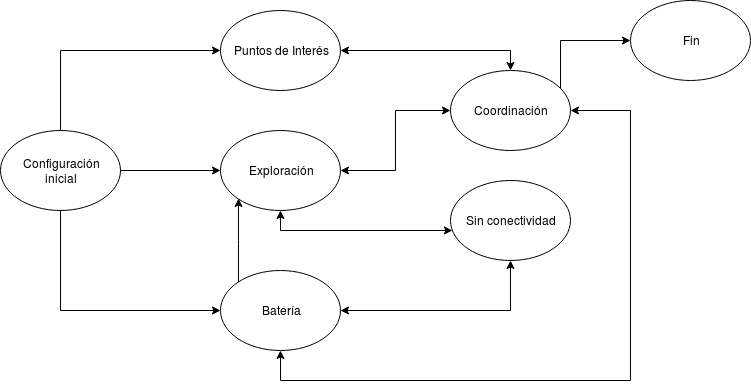
\includegraphics[width=.8\textwidth]{imagenes/chap5/image1}
	\caption{Máquina de estados simplificada.}
\end{figure}

\section{Máquina de Estados}
\subsection{Configuración inicial}

\begin{figure}[h!]
	\label{fig:comp}
	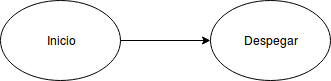
\includegraphics[width=.8\textwidth]{imagenes/chap5/image2}
	\caption{Especificación del estado Configuración inicial.}
\end{figure}

Al iniciar el sistema se realizan las configuraciones iniciales en el estado Inicio, donde se configuran las propiedades necesarias para la ejecución del sistema.
Es vital para el correcto funcionamiento del sistema establecer un canal de comunicación entre los drones que les permita intercambiar la información recabada a lo largo de la ejecución. La conexión entre los drones se implementa por medio de una arquitectura cliente-servidor, donde cada dron define al iniciar la ejecución del sistema un servidor TCP configurado para recibir la información de los demás drones y transmitirla a la máquina de estados. A su vez se define un cliente TCP para poder enviar los mensajes necesarios, siendo el mismo accesible desde los estados que requieran comunicarse con el resto de la flota
Existen varios propiedades parametrizables para la ejecución del sistema entre las que se incluyen:
las dimensiones del territorio a explorar 
las propiedades de la red wifi a la cual se conecta el dron
el tiempo total de ejecución del sistema
el algoritmo de exploración a utilizar
los puntos de interés a explorar
la altura a la que se mantiene el vuelo durante la exploración
activar funcionalidades complementarias como streaming de la exploración y el movimiento con rotación del dron
También se ejecuta un algoritmo de sincronización que permite a los drones comenzar la ejecución del resto de la máquina de estados al mismo tiempo. Esto permite que el tiempo de misión total de todos los drones sea el mismo y coordinar los tiempos en los que se deben visitar los puntos de interés.
Una vez concluida la etapa de inicio se procede al estado Despegar, donde se le envía al dron la instrucción de despegue y se determina cuál será el siguiente estado. 
\subsection {Exploración}

\begin{figure}[h!]
	\label{fig:comp}
	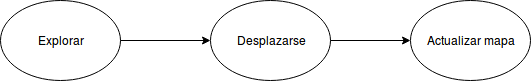
\includegraphics[width=.8\textwidth]{imagenes/chap5/image3}
	\caption{Especificación del estado Exploración.}
\end{figure}

La estrategia de exploración sigue el esquema de la Figura 3, donde se analiza para cada movimiento cuál es la nueva zona a visitar, consiguiendo de esta forma seguir un algoritmo que sea reactivo a la situación actual de la realidad tomando la mejor decisión en función de los datos recabados.
En el estado Explorar es donde se determina cual es el siguiente movimiento a realizar. Para calcular la próxima zona se cuenta con 2 alternativas, las cuales serán analizadas en la sección de experimentación para determinar cuál de ellas es más efectiva. Una de las alternativas diseñadas es utilizar un algoritmo greedy basado en determinar el siguiente movimiento en función de seleccionar entre las zonas vecinas, seleccionando aquella que fue visitada con mayor antelación o que nunca haya sido visitada. La otra opción es una variante del algoritmo descrito anteriormente, donde además se divide el territorio a explorar en diferentes regiones, por lo que al momento de determinar el siguiente movimiento no solo se consideran las zonas vecinas a la posición actual del dron, sino que también se realiza un control sobre el cubrimiento de las diferentes regiones del mapa determinando, en caso de ser necesario, desplazarse a una nueva región si la misma no cumple con las expectativas de la exploración.
Una vez determinado el siguiente movimiento a realizar se ejecuta el estado Desplazarse, donde se le envía al dron la instrucción de moverse hacia la posición calculada.
Al momento de finalizar el desplazamiento el dron cambia al estado Actualizar mapa, donde se registra la posición actual como visitada 

\subsection {Puntos de interés}

\begin{figure}[h!]
	\label{fig:comp}
	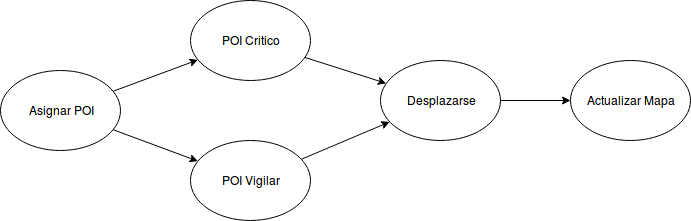
\includegraphics[width=.8\textwidth]{imagenes/chap5/image4}
	\caption{Especificación del estado Puntos de interés.}
\end{figure}

Cada punto de interés tiene un intervalo de tiempo asociado en el cual debe ser visitado por algún dron. En el caso de que no se cumpla con este requisito para algún punto de interés los drones entran en el estado Asignar POI, en el cual los drones eligen de forma conjunta a uno de ellos para que se encargue de ir a esa posición en forma prioritaria. Para tomar esta decisión los drones implementan un algoritmo de consenso basado en Paxos [27].



\subsubsection{Algoritmo de consenso}
Paxos es un algoritmo de consenso basado en el envío de mensajes que asegura un consenso entre N procesos participantes siempre y cuando se cumplan algunas condiciones:
La cantidad de procesos que fallan en algún momento del algoritmo no sea mayor o igual a N/2.
Los procesos pueden tener fallos pero no envían información incorrecta de forma intencional (no se producen fallos bizantinos).
Los procesos se envían mensajes asincrónicos que pueden tomar un tiempo indeterminado en llegar o directamente pueden perderse.
Si un mensaje llega a destino este no es corrupto, o si lo es se puede detectar.
Todos los procesos pueden enviarles mensajes a los demás de forma directa
Durante la ejecución del algoritmo no tiene porqué haber un proceso que actúe de líder, de hecho varios procesos pueden actuar como si fueran el líder, pero eventualmente se debe decidir un líder que dirima situaciones de conflicto.

En la implementación desarrollada del algoritmo todos los procesos actúan como líder hasta el final del proceso. Se define un líder solo en caso de que haya empates en la decisión final tomada y el líder se decide en base a la dirección IP de los drones: el dron que participa en el algoritmo que tenga el número más grande de IP es el líder. Se tomó esta decisión porque no todos los drones tienen porque participar en el algoritmo de consenso, solo lo hacen aquellos que se encuentren conectados a la red, tengan disponibilidad de batería y que no se encuentren en otra misión de alta prioridad. Esto lleva a que en cualquier ejecución del algoritmo de consenso pueda haber cualquier combinación de drones participando, por lo que se necesitaría un orden jerárquico completamente definido para establecer un líder desde el principio. Además los drones pueden perder conexión en cualquier momento del algoritmo, por lo que no resulta muy conveniente depender de que un único dron sea líder durante todo el proceso.

Además de la figura de líder, en un algoritmo Paxos se definen otros tres roles:
Proponentes: Son aquellos procesos que proponen valores para la decisión
Aceptadores: Son aquellos procesos que deciden aceptar o no los valores propuestos por los Proponentes
Receptores: Son aquellos procesos que no tomaron parte en el algoritmo de consenso y que deben ser informados de su resultado

La implementación propuesta hace que todos los drones participantes en la toma de decisión sean a la vez Proponentes y Aceptadores. De nuevo, esto se debe a que cualquier combinación de drones puede participar en el algoritmo y no existe un criterio objetivo para dictaminar quienes serán Proponentes o Aceptadores.

El algoritmo se divide en varias etapas:
Paso 1: Los drones que se encuentran disponibles (entendiéndose por disponible que tienen suficiente batería y no se encuentran realizando otras tareas prioritarias) le envían mensajes a todos los otros drones de la red informándoles de que quieren participar en la toma de decisión para el punto de interés correspondiente. Luego se quedan esperando durante un cierto tiempo configurable a que otros miembros de la red les envíen mensajes similares. De esta forma cada dron genera una lista con todos los drones participantes en la toma de decisión. Estos drones pasan a convertirse en los procesos participantes en la toma de decisión. Para evitar inconsistencias en la lista de participantes, la ventana de tiempo en la que los drones pueden mandar estos mensajes para participar se mide desde el momento en que el primer dron envía sus mensajes de participación. Esta técnica para sincronizar las ventanas de tiempo en las que se pueden enviar mensajes se usa en los otros pasos del algoritmo.
Paso 2: Una vez que se establece la lista de participantes todos los participantes se envían mensajes entre ellos informando de su distancia al punto de interés a atender. De nuevo, se establece una ventana de tiempo para la cual estos mensajes son válidos y que es absoluta para todos los drones.
Paso 3: Con la información obtenida en el paso 2 cada participante determina de forma independiente cual es el dron más cercano al punto de interés y envía un mensaje a los demás proponiendo a ese dron como candidato a vigilar el POI. Si existen dos drones que se encuentran a la misma distancia se elige al que tenga mayor valor de IP. Como siempre, se establece una ventana de tiempo absoluta para el envío de estos mensajes.
Paso 4: Cada proceso revisa las propuestas realizadas por todos los demás y aquella que fue propuesta más veces se convierte en la nueva decisión propuesta del proceso (de nuevo, si existen empates se elige al que tenga mayor valor de IP). Luego, cada proceso le comunica a los demás participantes esta nueva propuesta. Este paso se repite hasta que todos los procesos proponen la misma decisión, la cual se convierte en la decisión elegida. En la práctica, casi nunca es necesario repetir este paso.
Paso 5: Los procesos participantes le comunican a los drones Receptores la decisión tomada. Todos los drones pasan a monitorear al dron elegido para asegurarse de que cumpla su misión.

Dado que las distancias son valores absolutos todos los procesos que siguen el algoritmo de forma correcta deberían elegir al mismo dron en el paso 3 (esto sucede incluso en caso de empates en las distancias porque se dirime en base a las direcciones IP que también son absolutas y únicas) esto implica que para que se elija un dron erróneo en el paso 4 más de la mitad de los procesos deben de haber fallado en alguna parte del algoritmo. La única excepción a esta regla es si el dron elegido falla justo al final del paso 4 y piensa que no lo eligieron. Sin embargo todos los drones controlan de forma periódica que los puntos de interés asignados a algún dron efectivamente estén siendo vigilados, por lo tanto si se llega a dar este caso borde los otros drones lo detectan y se vuelve a realizar el proceso de selección.

Vigilancia de puntos de interés
Los drones que no fueron seleccionados en el estado Asignar POI vuelven al estado  Exploración. El dron seleccionado en cambio debe priorizar la visita de la zona asignada por lo que debe modificar la forma de seleccionar los desplazamientos a realizar. En caso de que no se haya superado el tiempo en que el punto de interés es considerado como crítico se ejecuta el estado POI Vigilar donde se realiza un conjunto de pasos similar al del comportamiento descrito en el estado Exploración con la principal diferencia que se consideran como zonas vecinas a visitar solo a aquellas donde su distancia con respecto al punto de interés es menor a la distancia de la ubicación actual, consiguiendo de esta forma disminuir la distancia en cada desplazamiento realizado.
Si se sobrepasa el tiempo establecido para considerar la zona a visitar como crítica sin que la misma haya sido visitada por algún miembro de la flota de exploración se realiza la ejecución del estado POI Crítico, en el cual el dron designado a explorar la zona se dirige a la misma directamente. Para determinar el camino a seguir para llegar al destino se utiliza el algoritmo A*(A aster) [28], el cual permite identificar el camino más corto en una red haciendo uso de la distancia de 
Manhattan (d((a1,b1),(a2,b2))=a2-a1+b2-b1 ) como función de heurística con el fín de etiquetar las zonas por las que se puede trasladar el dron para asignarle un valor que se utiliza para determinar si dicha zona puede formar parte del camino más corto, explorando en cada iteración los nodos vecinos a la zona actual y seleccionando como miembro de la solución a la zona con mejor valor asignado por la función de heurística.
Cuando se visita el punto de interés se reinicia el timer con el tiempo configurado para que la zona vuelva a ser visitada más adelante y se envía un mensaje a los demás drones para que estos también restablezcan su timer para el punto de interés.



\subsection {Batería}


\begin{figure}[h!]
	\label{fig:comp}
	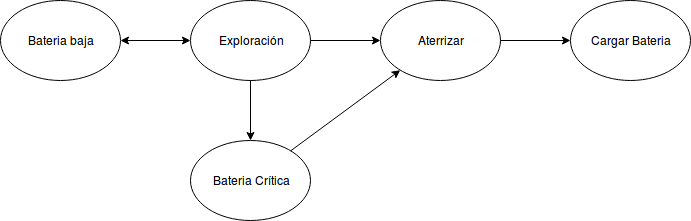
\includegraphics[width=.8\textwidth]{imagenes/chap5/image5}
	\caption{Especificación del estado Bateria.}
\end{figure}

Esta sección de la máquina de estados se encarga de controlar el estado de la batería del dron con el principal objetivo de evitar que el mismo se quede sin carga en la exploración y deba realizar un aterrizaje forzoso sin control del sistema implementado.
Para esto se realiza un chequeo del porcentaje de carga de la  batería y en caso de encontrarse la misma por debajo del 20% se cambia al estado Batería baja. Una vez que el dron se sitúa en este estado el mismo realiza las tareas del estado Exploración descrito anteriormente, con la diferencia de que para determinar la siguiente zona a visitar se consideran como válidas sólo las zonas que se encuentran más cerca de la base con respecto al punto donde se encuentra actualmente, consiguiendo de esta forma reducir en cada movimiento la distancia con respecto a la estación de carga.
A su vez también se realiza un control sobre la distancia entre el dron y la estación de carga y se compara la misma con la cantidad de movimientos necesarios para volver a la estación de carga de forma directa. En caso de que la cantidad de movimientos para volver a la estación de carga sea igual a la cantidad de movimientos restantes más una cantidad predefinida de movimientos se pasa al estado Bateria crítica, donde el dron abandona la exploración y se dirige a la estación de carga. 
Para calcular la distancia a la estación de carga y el camino a seguir se hace uso del algoritmo A*(A aster).
Una vez que el dron llega a la estación de carga pasa al estado Aterrizar, donde se ejecutan las instrucciones para realizar el procedimiento de aterrizaje seguro para más adelante activar el estado Cargar batería. Cuando se termina la carga de la batería el dron vuelve a realizar las tareas de exploración.
\subsection {Coordinación}


\begin{figure}[h!]
	\label{fig:comp}
	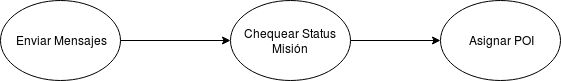
\includegraphics[width=.8\textwidth]{imagenes/chap5/image6}
	\caption{Especificación del estado Coordinación.}
\end{figure}

En esta etapa se realizan las actividades de comunicación de la flota de exploración para optimizar la estrategia a seguir.
Cuando un dron se encuentra en el estado Enviar Mensajes se comunica por medio de la conexión establecida en la Configuración Inicial con los demás miembros de la flota para transmitirle la zona del mapa en la que se encuentra actualmente. De esta forma los demás drones marcan la zona recibida como visitada.
Por otra parte se controla el estado de la vigilancia de los puntos de interés asignadas a otros miembros de la flota, para esto al momento de asignar un punto de interés a un dron se programa una tarea de chequeo a realizar en un período de tiempo preestablecido (el mismo es configurable) cambiando al estado Chequear Status Misión, donde todos los drones disponibles buscan establecer una conexión con el dron que tiene la misión de vigilar la zona asignada. Cuando se recibe una respuesta satisfactoria del dron que se encuentra encargado de la misión se les envía un mensaje a los demás drones para avisarles que la misión está siendo ejecutada con éxito. En caso de que ningún miembro de la flota pueda recibir una respuesta por parte del dron con la misión asignada se determina que la misma fue cancelada y se pasa al estado Asignar POI para reasignar el punto de interés a un nuevo dron disponible.
\subsection {Sin conectividad}


\begin{figure}[h!]
	\label{fig:comp}
	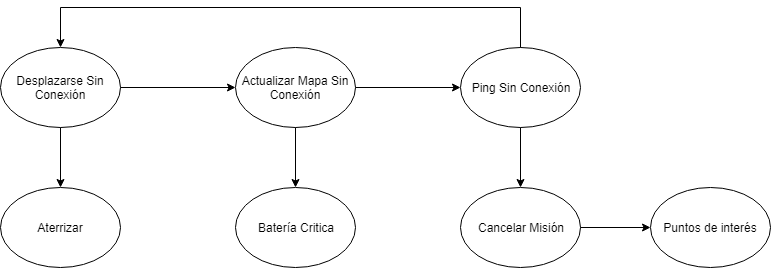
\includegraphics[width=.8\textwidth]{imagenes/chap5/image7}
	\caption{Especificación del estado Sin conectividad.}
\end{figure}

En caso de que el dron no pueda establecer un canal de comunicación con ningún otro miembro de la flota se declara a sí mismo sin conectividad e inicia la ejecución de los estados que se muestran en la Figura 7.
El primer estado en ser ejecutado es Desplazarse Sin Conexión, donde se sigue una estrategia de movimientos similar a la del estado Exploración, con la particularidad de decidir las siguientes zonas a visitar buscando disminuir la distancia con la base, con la finalidad de poder recuperar la conexión con algún dron.
Una vez que el dron haya terminado de desplazarse hacia la nueva zona se cambia el estado a Actualizar Mapa Sin Conexión, donde se actualiza la zona como visitada y se guarda la posición para poder enviarla al resto de la flota en caso de poder restablecer la conexión más adelante.
En el estado Ping Sin Conexión se chequea si se recupero la conexión buscando establecer una comunicación con algún otro dron, en caso de no tener éxito se retorna al estado Desplazarse Sin Conexión, en cambio, si se obtiene una respuesta de otro dron se abandona el modo Sin Conectividad  para volver al funcionamiento habitual.
Si el dron previo a la pérdida de la conectividad tenía asignado un punto de interés se ejecuta el estado Cancelar Misión, donde se enviá un mensaje a los demás drones comunicando que se debe reasignar el punto de interés para posteriormente ejecutar las acciones de Puntos de Interés descritas anteriormente.
En caso de no recuperar la conectividad y llegar a la base se ejecuta el estado Aterrizar para finalizar su ejecución del sistema.
Al igual que cuando se tiene conexión se realiza un control sobre el porcentaje de carga de la batería y se ejecuta el estado Batería Crítica de la misma forma que se describe en la sección Batería.
\subsection {Fin}


\begin{figure}[h!]
	\label{fig:comp}
	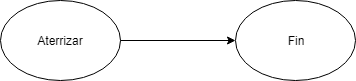
\includegraphics[width=.8\textwidth]{imagenes/chap5/image8}
	\caption{Especificación del estado Fin.}
\end{figure}


Al finalizar la ejecución del sistema se procede al aterrizaje del dron en la base para posteriormente ejecutar el estado Fin donde se cierra el canal de comunicación y se registra la información relevante de la ejecución en archivos con formato csv.
\section{Funcionalidades complementarias}
El sistema desarrollado cuenta con funcionalidades opcionales que se incorporaron en función de considerarse útiles para algunos escenarios de uso particulares.
\subsection{Streaming}
En caso de querer hacer uso del sistema para la vigilancia de un terreno es de gran utilidad poder visualizar desde un centro de control los datos obtenidos por la cámara de los drones.
Por esta razón se incorpora la funcionalidad de poder transmitir en vivo la grabación realizada durante la exploración. Para esto basta con estar conectado a la red wifi en la que se encuentra el dron y recibir los datos enviados por el mismo mediante una conexión UDP en el puerto 4444, estos datos pueden ser visualizados directamente haciendo uso de un reproductor de video (fue verificado con el programa VLC).
Modo de navegación
Al momento de determinar el modo en el que los movimientos de los drones se pueden realizar se analizaron dos alternativas, una que consiste en realizar todos los movimientos sin realizar giros ejecutando desplazamientos de forma lateral en caso de querer moverse hacia un costado, y otra en la que todos los desplazamientos se ejecutan hacia adelante realizando previamente el giro correspondiente.
En función del tiempo necesario para ejecutar los movimientos de rotación se optó por incluir como configuración por defecto no realizar los mismos.
En caso de querer realizar giros en los desplazamientos, lo cual puede resultar útil si se desea activar el streaming de la exploración, es posible activarlo configurando el parámetro correspondiente.

\subsection{Auditoría de la exploración}
Para determinar si la ejecución del sistema cumplió con los objetivos establecidos se incorpora la posibilidad de almacenar en cada dron de la flota de exploración un archivo que contiene estadśiticas detallando el porcentaje de mapa cubierto, la cantidad de puntos de interés visitados y los tiempos de respuesta para las mismas. 
Esta funcionalidad es particularmente útil para la evaluación experimental realizada en la investigación.
\subsection{Altura de vuelo}
Dependiendo de las características del terreno a explorar puede ser necesario configurar a qué altura se debe realizar la exploración. Configurar la altura de vuelo consiste en asignar el rango de altura permitido en metros.
Para determinar la altura a la que se encuentra el dron se utiliza la información publicada por el mismo, la cual hace uso de un sensor para determinar la misma siempre que esta sea menor a 5 metros y cálculos con el GPS para el resto de los casos. 
 % Se carga el capítulo 05
  \chapter{Experimentación}

\section {Casos de prueba}
A continuación se describe la metodología utilizada para la evaluación experimental de las diferentes variaciones de los algoritmos de exploración. Las pruebas se realizaron de forma automatizada con el simulador Sphinx para drones de la marca Parrot. La flota consta de dos drones.

En total se cuenta con tres estrategias de exploración diferentes a evaluar. Como ya se discutió en otras secciones los algoritmos greedy son los de mayor prevalencia para resolver problemas de múltiples agentes ya que no requieren grandes capacidades computacionales y han demostrado en muchos experimentos que tienen desempeños iguales o mejores a otros tipos de algoritmos en teoría más complejos. De esta forma se optó por evaluar el algoritmo greedy contra el algoritmo basado en distribución de zonas para determinar si los algoritmos greedy resultan convenientes para resolver este problema en particular. La tercera estrategia a evaluar es un algoritmo de funcionamiento aleatorio, es decir, un algoritmo que define todos los movimientos del dron de forma aleatoria. Este algoritmo aleatorio sirve como prueba de control y los otros algoritmos deberían tener mejores rendimientos que el suyo para poder considerarse viables.

Para cada uno de los algoritmos se relevaron varias medidas. Los algoritmos cuentan con dos objetivos principales: en primer lugar deben cubrir toda la zona a explorar de la forma más homogénea y rápida posible y luego deben atender los puntos de interés con la menor demora posible. Esto lleva a que los datos relevados también se separen en dos categorías, cada una corresponde a uno de estos objetivos.
Para medir el cubrimiento del mapa se releva el porcentaje del área que fue explorada en función del tiempo, tomándose una medición cada 10 segundos y además se registra la cantidad de veces que los drones pasaron por cada ubicación del área.
Para medir el nivel de atención de los puntos de interés se releva la cantidad de veces que se desencadenó una interrupción para atender un punto de interés, si esa interrupción es de tipo normal o crítica, la cantidad de interrupciones que los drones efectivamente atendieron y cuanto tiempo demoraron en atenderla. Para cada de uno de estos registros también se releva cual fue el punto de interés al que corresponde.

El siguiente paso fue el de crear instancias de prueba sobre los que ejecutar los algoritmos. Para esto se optó por crear escenarios que sean realistas y que representen realidades diferentes, de esta forma se puede evaluar el desempeño de los algoritmos en situaciones variadas. Se diseñaron tres escenarios de diferente tamaño y con obstáculos de diferente tipo y distribución, luego para cada escenario se crearon diez instancias con variaciones aleatorias, esto permite evaluar los escenarios con menor sesgo. Las instancias difieren entre sí en la ubicación de sus puntos de interés y en el tiempo que deben ser atendidos. De esta forma podemos evaluar si existen puntos en cada escenario que resulten más difíciles de controlar. En total, cada algoritmo fue evaluado cuatro veces en cada instancia de cada escenario.
El primer escenario consiste en un galpón de aproximadamente 5000 m2. En este escenario los principales obstáculos vienen dados por paredes y racks que también forman estructuras en forma de pared. El galpón tiene una única entrada que representa un punto de interés a vigilar. Su ubicación y la frecuencia con la que debe ser atendido varía en cada instancia del escenario.

\begin{figure}[h!]
	\label{fig:comp}
	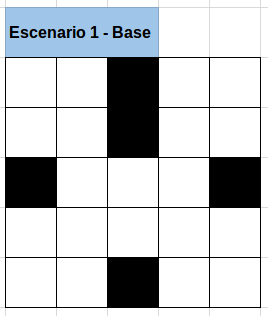
\includegraphics[width=.8\textwidth]{imagenes/chap6/image1}
	\caption{Versión base del escenario 1.}
\end{figure}

El segundo escenario consiste de un establecimiento que ocupe una cuadra entera (aproximadamente 10000 m2) compuesto por tres edificios principales y el resto del mapa es una zona de patio despejada. Los edificios definen zonas prohibidas en las que los drones no pueden entrar. En este escenario se cuenta con tres puntos de interés que representan diferentes zonas de ingreso al predio.


\begin{figure}[h!]
	\label{fig:comp}
	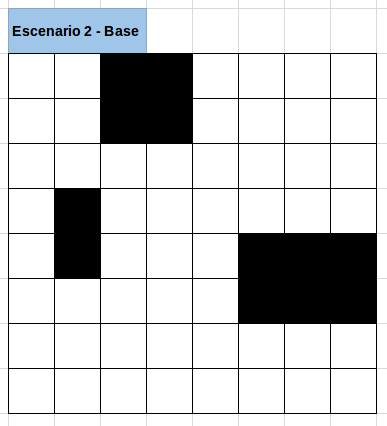
\includegraphics[width=.8\textwidth]{imagenes/chap6/image2}
	\caption{Versión base del escenario 2.}
\end{figure}

El último escenario consiste en un campo de 2 hectáreas (aproximadamente 20000 m2) en el cual hay solo algunos obstáculos aislados en forma de árboles y casas. En este caso se cuenta con cinco puntos de interés que representan corrales, puntos de entrada o la casa del dueño.


\begin{figure}[h!]
	\label{fig:comp}
	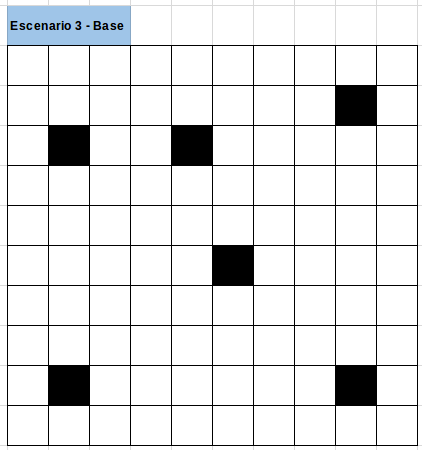
\includegraphics[width=.8\textwidth]{imagenes/chap6/image3}
	\caption{Versión base del escenario 3.}
\end{figure}

Por último se establecieron algunos datos paramétricos de interés.
La altura de vuelo se definió en 10 metros ya que a esta altura se pueden esquivar la mayoría de los obstáculos (solo hay que preocuparse por obstáculos mayores y estáticos como paredes, árboles o edificios) pero a su vez es lo suficientemente cercano al suelo para no perder calidad de imagen de la cámara, de esta forma se puede vigilar la zona de forma efectiva.
Para los drones Bebop 2 una altura de vuelo de 10 metros implica que se tiene un área de visión de 10x18 metros con la cámara apuntando directamente hacia abajo. Esto permite definir la unidad con la que se divide la matriz del área a explorar como un rectángulo de 10x18 metros. De esta forma el escenario 1 queda representado como una matriz de 5x5 unidades, el escenario 2 se representa como uno de 8x8 unidades y el escenario 3 se representa como uno de 10x10 unidades.
Se estableció un tiempo de misión de 20 minutos ya que este es un tiempo un poco menor a los 25 minutos de duración de la batería. Esto permite obtener mediciones de cuanto se puede explorar con una carga de batería dejando un colchón de 5 minutos para imprevistos.
Todos los drones despegan desde la misma ubicación, la cual representa la base a la que tienen que retornar cuando acabe la misión o en caso de emergencia.

A continuación se presenta un resumen de las características mencionadas de la evaluación experimental:


Algoritmos evaluados
Aleatorio
Este algoritmo determina los movimientos del dron de forma completamente aleatoria. Sirve principalmente como prueba de control.
Greedy basado en timestamps
Un algoritmo greedy que determina el siguiente movimiento del dron en base al tiempo que pasó desde la última vez que un dron visitó los puntos adyacentes a la posición actual en el mapa.
No greedy basado en timestamps
Un algoritmo que divide el mapa en regiones. Un dron explora una misma región hasta que esta se encuentre mayormente explorada o hasta que se detecta que hay otras por las que la flota no pasa desde hace mucho tiempo. Luego cambia de región y repite el proceso.
Tabla 2: Algoritmos evaluados























Escenario 1
Descripción
Un galpón o establecimiento de tamaño intermedio
Dimensiones físicas
5000 m2
Representación
Matriz de 5x5 unidades
Puntos de interés
1
Obstáculos
En forma de paredes
Escenario 2
Descripción
Un establecimiento de tamaño mayor que ocupe una cuadra entera
Dimensiones físicas
10000  m2
Representación
Matriz de 8x8 unidades
Puntos de interés
3
Obstáculos
En forma de zonas prohibidas
Escenario 3
Descripción
Un terreno o campo de 2 hectáreas
Dimensiones físicas
20000  m2
Representación
Matriz de 10x10 unidades
Puntos de interés
5
Obstáculos
En forma de puntos aislados
Tabla 3: Descripción de escenarios


Instancias
Instancias por escenario
10
Cantidad de ejecuciones por instancia y por algoritmo
4
Posición de los POI
Aleatoria
Frecuencia de atención de los POI
Aleatoria
Tabla 4: Descripción de instancias


Datos paramétricos
Cantidad de drones
2
Altura de vuelo
10 metros
Tamaño de la unidad de vuelo
10x18 metros
Tiempo de misión
20 minutos
Zona de despegue
Una única base en la posición (0,0) de cada mapa
Tabla 5: Datos paramétricos

Especificaciones técnicas
Tiempo total de simulación
120 horas
Sistema operativo
Ubuntu 16.04 64 bits
Procesador
Intel® Core™ i7-4510U CPU @ 2.00GHz × 4
Memoria RAM
8GB
Tarjeta gráfica
Intel® Haswell Mobile
Simulador
Sphinx 0.29.1, Gazebo 7.0.1
Tabla 6: Especificaciones técnicas

Resultados
FALTA ANALIZAR RESULTADOS

 % Se carga el capítulo 05
  \chapter{Conclusiones}

Dadas las limitantes encontradas en el Parrot Bebop 2 se destaca el hecho de haber sido posible ejecutar código de forma nativa por medio del lenguaje de scripting Python, generando una versión portable del mismo que puede ser trasladada a demás drones y dispositivos que cuenten con la arquitectura ARMv7 en su CPU. Esto no solo expande las posibilidades del trabajo realizado por el equipo, sino también de la comunidad de desarrolladores que a partir de este sistema pueden expandir las aplicaciones implementadas que se ejecutan directamente en los drones.
A su vez se encontró la dificultad de no poder implementar la conectividad de los drones por medio de una red ad-hoc que era uno de los objetivos propuestos al iniciar el trabajo. El obstáculo que impidió cumplir esta meta fue la limitación que otorga el dron a modificar su configuración por defecto. A pesar de esto se consiguió desarrollar una alternativa por medio de establecer un canal de comunicación entre los drones a través de una red wifi que se considera que se adapta al objetivo inicialmente planteado, destacando la facilidad de uso para el usuario final dado que es suficiente con presionar tres veces el botón de apagado del dron para modificar el modo de la interfaz wifi y conectarse a una red configurada.
La facilidad de instalación de las soluciones provistas tanto para ejecutar código en el dron como para establecer la conexión a la red wifi genera que el proceso de implantación del sistema en un dron que se encuentre en estado de fábrica sea extremadamente sencillo, dado que el mismo consiste en la copia de archivos al dron y la ejecución de un script. Esto puede resultar extremadamente útil si se desea utilizar una flota cuantiosa de drones para realizar la exploración de un territorio.
Sin embargo el principal problema encontrado fue el de conseguir determinar la ubicación del dron durante la ejecución del sistema. La alternativa empleada durante la investigación fue la de utilizar un posicionamiento relativo del dron en función de los movimientos realizados, lo cual no consigue los resultados de precisión esperados. Se analizaron otras posibilidades pero ninguna llegó a mejorar los resultados obtenidos con la solución seleccionada y por este motivo fueron descartados. Se concluye que el mayor problema reside en la falta de sensores equipados en el Parrot Bebop 2 que permitan realizar mediciones de distancia con respecto a objetos. La mejor alternativa en términos de precisión alcanzados, es la que incluye el procesamiento de las imágenes recabadas por la cámara del dron pero esto implica un costo extra en términos de recursos de hardware del dron que no se ha demostrado que sea capaz de soportar. Sí existen en cambio soluciones que realizan este procesamiento de forma remota haciendo uso de una base central que procese las imágenes con mayor capacidad de cómputo que los drones.
FALTA CONCLUIR EVALUACIÓN EXPERIMENTAL

 % Se carga el capítulo 05
  \chapter{Consideraciones finales}

\section{Título de sección}

Ejemplo de tabla

\begin{table}[h!]
	\centering
	\caption{Leyenda de tabla.}
	\label{tab:comp}
	\begin{tabular}{|c|c|c|}
		\hline
		$t$ (seg) & $x$(t) & $y$(t)\\
		\hline
		1 & 0.0000 & 0.0001\\
		2 & 0.5000 & 0.2498\\
		3 & 1.0000 & 1.0000\\
		4 & 1.5000 & 2.2403\\
		5 & 2.0000 & 4.0010\\
		6 & 2.5000 & 6.2459\\
		\hline
	\end{tabular}
\end{table}

Ejemplo de figura.

\begin{figure}[h!]
	\label{fig:comp}
	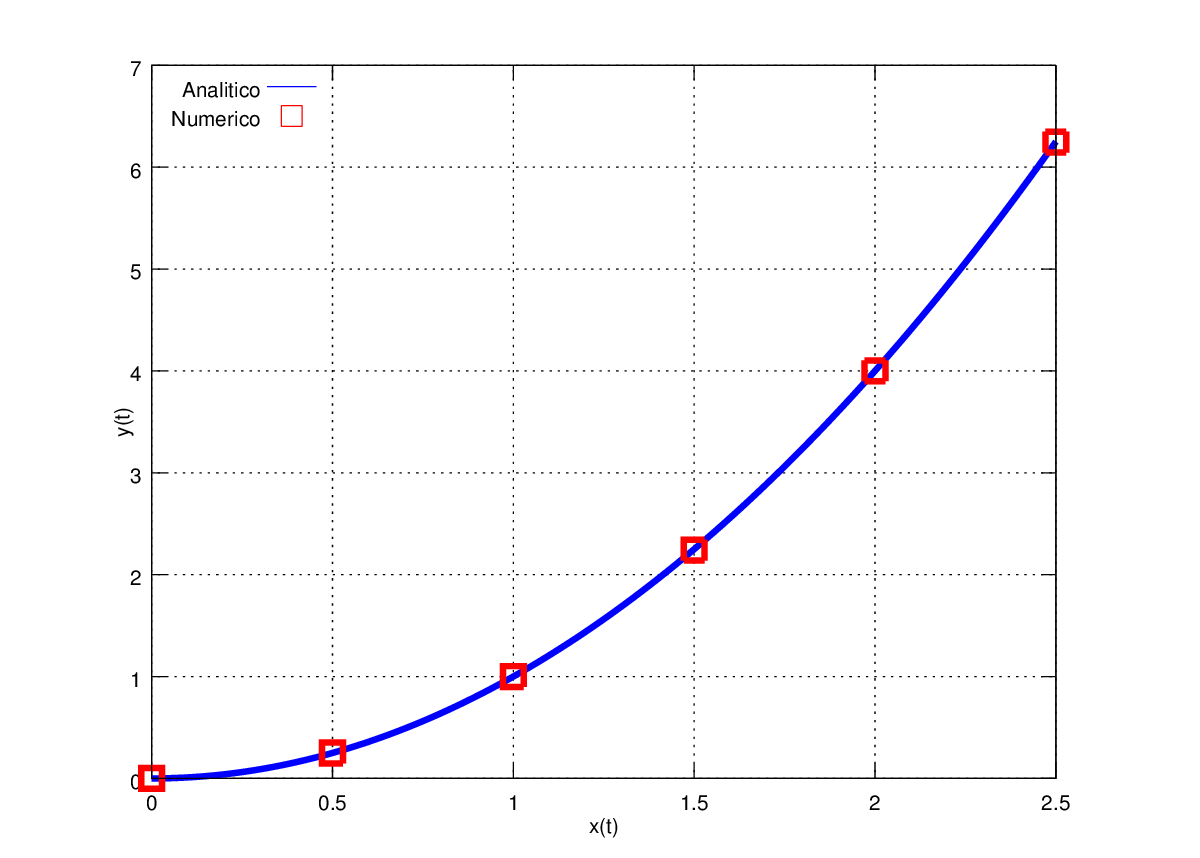
\includegraphics[width=.8\textwidth]{imagenes/chap4/x_vs_y}
	\caption{Leyenda de figura.}
\end{figure}
Ejemplo de ecuación:
\begin{equation}
y(x)=x^2
\end{equation}
En este capítulo se sintetizan las posturas expuestas en el capítulo anterior. Se retoma la pregunta de investigación y se expresa si los resultados apoyan o no la hipótesis planteada. 

Además, se pueden hacer contribuciones teóricas o metodológicas a la disciplina y recomendaciones para trabajos futuros o para profundizar en el campo, plantear nuevas interrogantes o proponer explicaciones \textit{post hoc}. En algunos trabajos este capítulo se subdivide en otras secciones que presentan algunos de los contenidos mencionados. 
En algunas tradiciones académicas este capítulo recibe distintas denominaciones: \textit{Conclusiones}, \textit{Conclusiones y trabajos a futuro}, \textit{Consideraciones finales y recomendaciones}. 

 % Se carga el capítulo 05
 % Seguir copiando la linea de arriba para agregar más capítulos.
  
  \backmatter % Comando que generalos apéndices, anexos y bibliografía. NO COMENTAR
  
  \bibliography{bibliografia/biblio_1,bibliografia/biblio_2} % Agregar la cantidad de archivos .bib que se tengan para la bibliografía.
  \bibend % No comentar
  % 
  \glosario 		         % Glosario, NO comentar
  %
  \apenarabicnumbering
  \apenmatter				 % Apéndices, NO comentar
  \chapter{Datos procesados}


  \chapter{Imágenes remasterizadas}\label{Ape2}

  \chapter{Entrevistas desgrabadas}\label{Ape3}

  % Seguir copiando la linea de arriba para agregar más apéndices.
  %
  \anexarabicnumbering
  \anexmatter				 % Anexos, NO comentar
  \chapter{Material legislativo}\label{Ane1}

XXXXX
  % Seguir copiando la linea de arriba para agregar más anexos.
  % 
\end{document}

% ===== FIN DEL DOCUMENTO =====